\documentclass[xcolor=x11names, compress]{beamer}

%% General document %%%%%%%%%%%%%%%%%%%%%%%%%%%%%%%%%%
\usepackage{graphicx}
\graphicspath{{graphics/}}

\usepackage{tikz}
\usepackage{color}
\input{rgb}

\definecolor{capri}{rgb}{0,.75,1}
\definecolor{coral}{rgb}{1,.2,.2}

\newcommand{\hltyellow}[1]{\colorbox{yellow}{$\displaystyle #1$}}
\newcommand{\hltblue}[1]{\colorbox{capri}{$\displaystyle #1$}}
\newcommand{\hltred}[1]{\colorbox{coral}{$\displaystyle #1$}}
\newcommand{\hltgreen}[1]{\colorbox{green}{$\displaystyle #1$}}

\usepackage{hyperref}

\usepackage{ulem}
\renewcommand<>{\sout}[1]{
  \only#2{\beameroriginal{\sout}{#1}}
  \invisible#2{#1}
}

%%%%%%%%%%%%%%%%%%%%%%%%%%%%%%%%%%%%%%%%%%%%%%%%%%%%%%

%% Beamer Layout %%%%%%%%%%%%%%%%%%%%%%%%%%%%%%%%%%
% \usetheme{Madrid}

\useoutertheme[subsection=false,shadow]{miniframes}
\useinnertheme{default}
\usefonttheme{serif}
\usepackage{palatino}

\setbeamerfont{title like}{shape=\scshape}
\setbeamerfont{frametitle}{shape=\scshape, series = \bfseries}
\setbeamertemplate{frametitle}[default][center]
\setbeamerfont{footnote}{size=\tiny}
\addtobeamertemplate{footnote}{}{\vspace{1ex}} %so that the footnotes do not overlap with navigation symbols at bottom

\setbeamercolor*{lower separation line head}{bg=DeepSkyBlue4} 
\setbeamercolor*{normal text}{fg=black,bg=white} 
\setbeamercolor*{alerted text}{fg=red} 
\setbeamercolor*{example text}{fg=black} 
\setbeamercolor*{structure}{fg=black}
 
\setbeamercolor*{palette tertiary}{fg=black,bg=black!10} 
\setbeamercolor*{palette quaternary}{fg=black,bg=black!10} 

\renewcommand{\(}{\begin{columns}}
\renewcommand{\)}{\end{columns}}
\newcommand{\<}[1]{\begin{column}{#1}}
\renewcommand{\>}{\end{column}}

\def\signed #1{{\leavevmode\unskip\nobreak\hfil\penalty50\hskip2em
  \hbox{}\nobreak\hfil(#1)%
  \parfillskip=0pt \finalhyphendemerits=0 \endgraf}}

\newsavebox\mybox
\newenvironment{aquote}[1]
  {\savebox\mybox{#1}\begin{quote}}
  {\signed{\usebox\mybox}\end{quote}}


%%%%%%%%%%%%%%%%%%%%%%%%%%%%%%%%%%%%%%%%%%%%%%%%%%%%

\begin{document}


%%%%%%%%%%%%%%%%%%%%%%%%%%%%%%%%%%%%%%%%%%%%%%%%%%%%%%
{
  \usebackgroundtemplate{\includegraphics[width=\paperwidth]{back.jpg}}
\begin{frame}[plain]

  \vspace{100pt}
  \title{\bf Selection -- \\Mutualistic Networks}

\author{
	Samraat Pawar\\
	\vspace{5pt}
	\url{www.pawarlab.org}\\
	\vspace{5pt}
	{\it  Department of Life Sciences, Silwood Park Campus}\\
Imperial College London\\
  \vspace{5pt}
\today
  % \centering
  % \includegraphics[height = .3.3in]{Imperial_Color1.pdf}
}
 
\titlepage
\date{} 

\end{frame}
}

%%%%%%%%%%%%%%%%%%%%%%%%%%%%%%%%%%%%%%%%%%%%%%%%%%%%%%
\section{\scshape Introduction}
% \subsection{}
%%%%%%%%%%%%%%%%%%%%%%%%%%%%%%%%%%%%%%%%%%%%%%%%%%%%%%

\begin{frame}{Outline}
  \begin{itemize}\setlength{\itemindent}{0em}\itemsep12pt

    \item Introduction

    \item Overview of Mutualistic Networks

    \item Structure and Stability
    
    \item Summary, Questions, and Readings

  \end{itemize}  

\end{frame}


%%%%%%%%%%%%%%%%%%%%%%%%%%%%%%%%%%%%%%%%%%%%%%%%%%%%%%
\begin{frame}{Recall: Ecological Networks}

  \begin{columns}[c]
    \column{0.6\textwidth}
    \begin{itemize}[<+->]\setlength{\itemindent}{0em} \itemsep6pt
      \item {\bf Ecological Network}: Network of interactions where {\it nodes} ($\boldsymbol{\cdot}$) are individuals or (usually, species') populations, and {\it links} (---) the interactions between pairs of nodes 
    \end{itemize}
    \column{0.4\textwidth}\centering
    {\footnotesize The Silwood Park Food web}\\
    \vspace{3pt}
    \includegraphics[width=.7\linewidth]{SilwoodWeb.png}
  \end{columns}
  \pause 
  \vspace{6pt}
  \begin{itemize} \setlength{\itemindent}{-1em}
    \item Types:
    \begin{itemize}\setlength{\itemindent}{-2em}\itemsep10pt
    \item Trophic networks ($+/-$) (e.g., food webs)
    \item {\bf Mutualistic networks ($+/+$) (e.g., plant-pollinator networks)}    
    \item Competitive networks ($-/-$) (e.g., plant-plant or microbe-microbe)
    \item Behavioural networks ($+/-$, $+/+$,$+/-$ ) (e.g., social networks)
   \end{itemize} 
  \end{itemize}
  
  \end{frame}

%%%%%%%%%%%%%%%%%%%%%%%%%%%%%%%%%%%%%%%%%%%%%%%%%%%%%%
\section{\scshape Mutualistic Networks}
%%%%%%%%%%%%%%%%%%%%%%%%%%%%%%%%%%%%%%%%%%%%%%%%%%%%%

%%%%%%%%%%%%%%%%%%%%%%%%%%%%%%%%%%%%%%%%%%%%%%%%%%%%%%
\begin{frame}{Mutualistic Networks}

  \begin{itemize}[<+->]\setlength{\itemindent}{0em} \itemsep3pt
    \item {\bf Mutualistic Networks}: Network of interactions made of pairs of individuals or (usually species') populations {\it mutually benefiting} each other
    \item The benefit can be through direct exchange of matter/energy/metabolites/nutrients 
      \begin{itemize}\setlength{\itemindent}{-1em} 
        \item Plant-fungal (especially, Mycorrhizal) soil interaction networks
        \item Bacterial interaction networks---mutualisms can develop by exchange of organic substrates/metabolites between populations (e.g., Yogurt and Cheese!)
      \end{itemize} 
      \item Or through combination of direct and indirect benefits
      \begin{itemize}\setlength{\itemindent}{-1em} 
        \item Plant-Pollinator Networks: Pollination is an indirect benefit to the plant, nectar is a direct (energy) to the pollinator
        \item Plant-Animal seed dispersal Networks: Also an indirect-direct benefit combination 
        \item Ant-Plant association networks: Plant gets protection (direct, but non-energy benefit), Ants get nectar (energy) 
      \end{itemize}
  \end{itemize}

\end{frame}

%%%%%%%%%%%%%%%%%%%%%%%%%%%%%%%%%%%%%%%%%%%%%%%%%%%%%%
\begin{frame}{Origin of Mutualistic networks}

  \begin{center}
    
  \begin{tikzpicture}
    \node (img1) {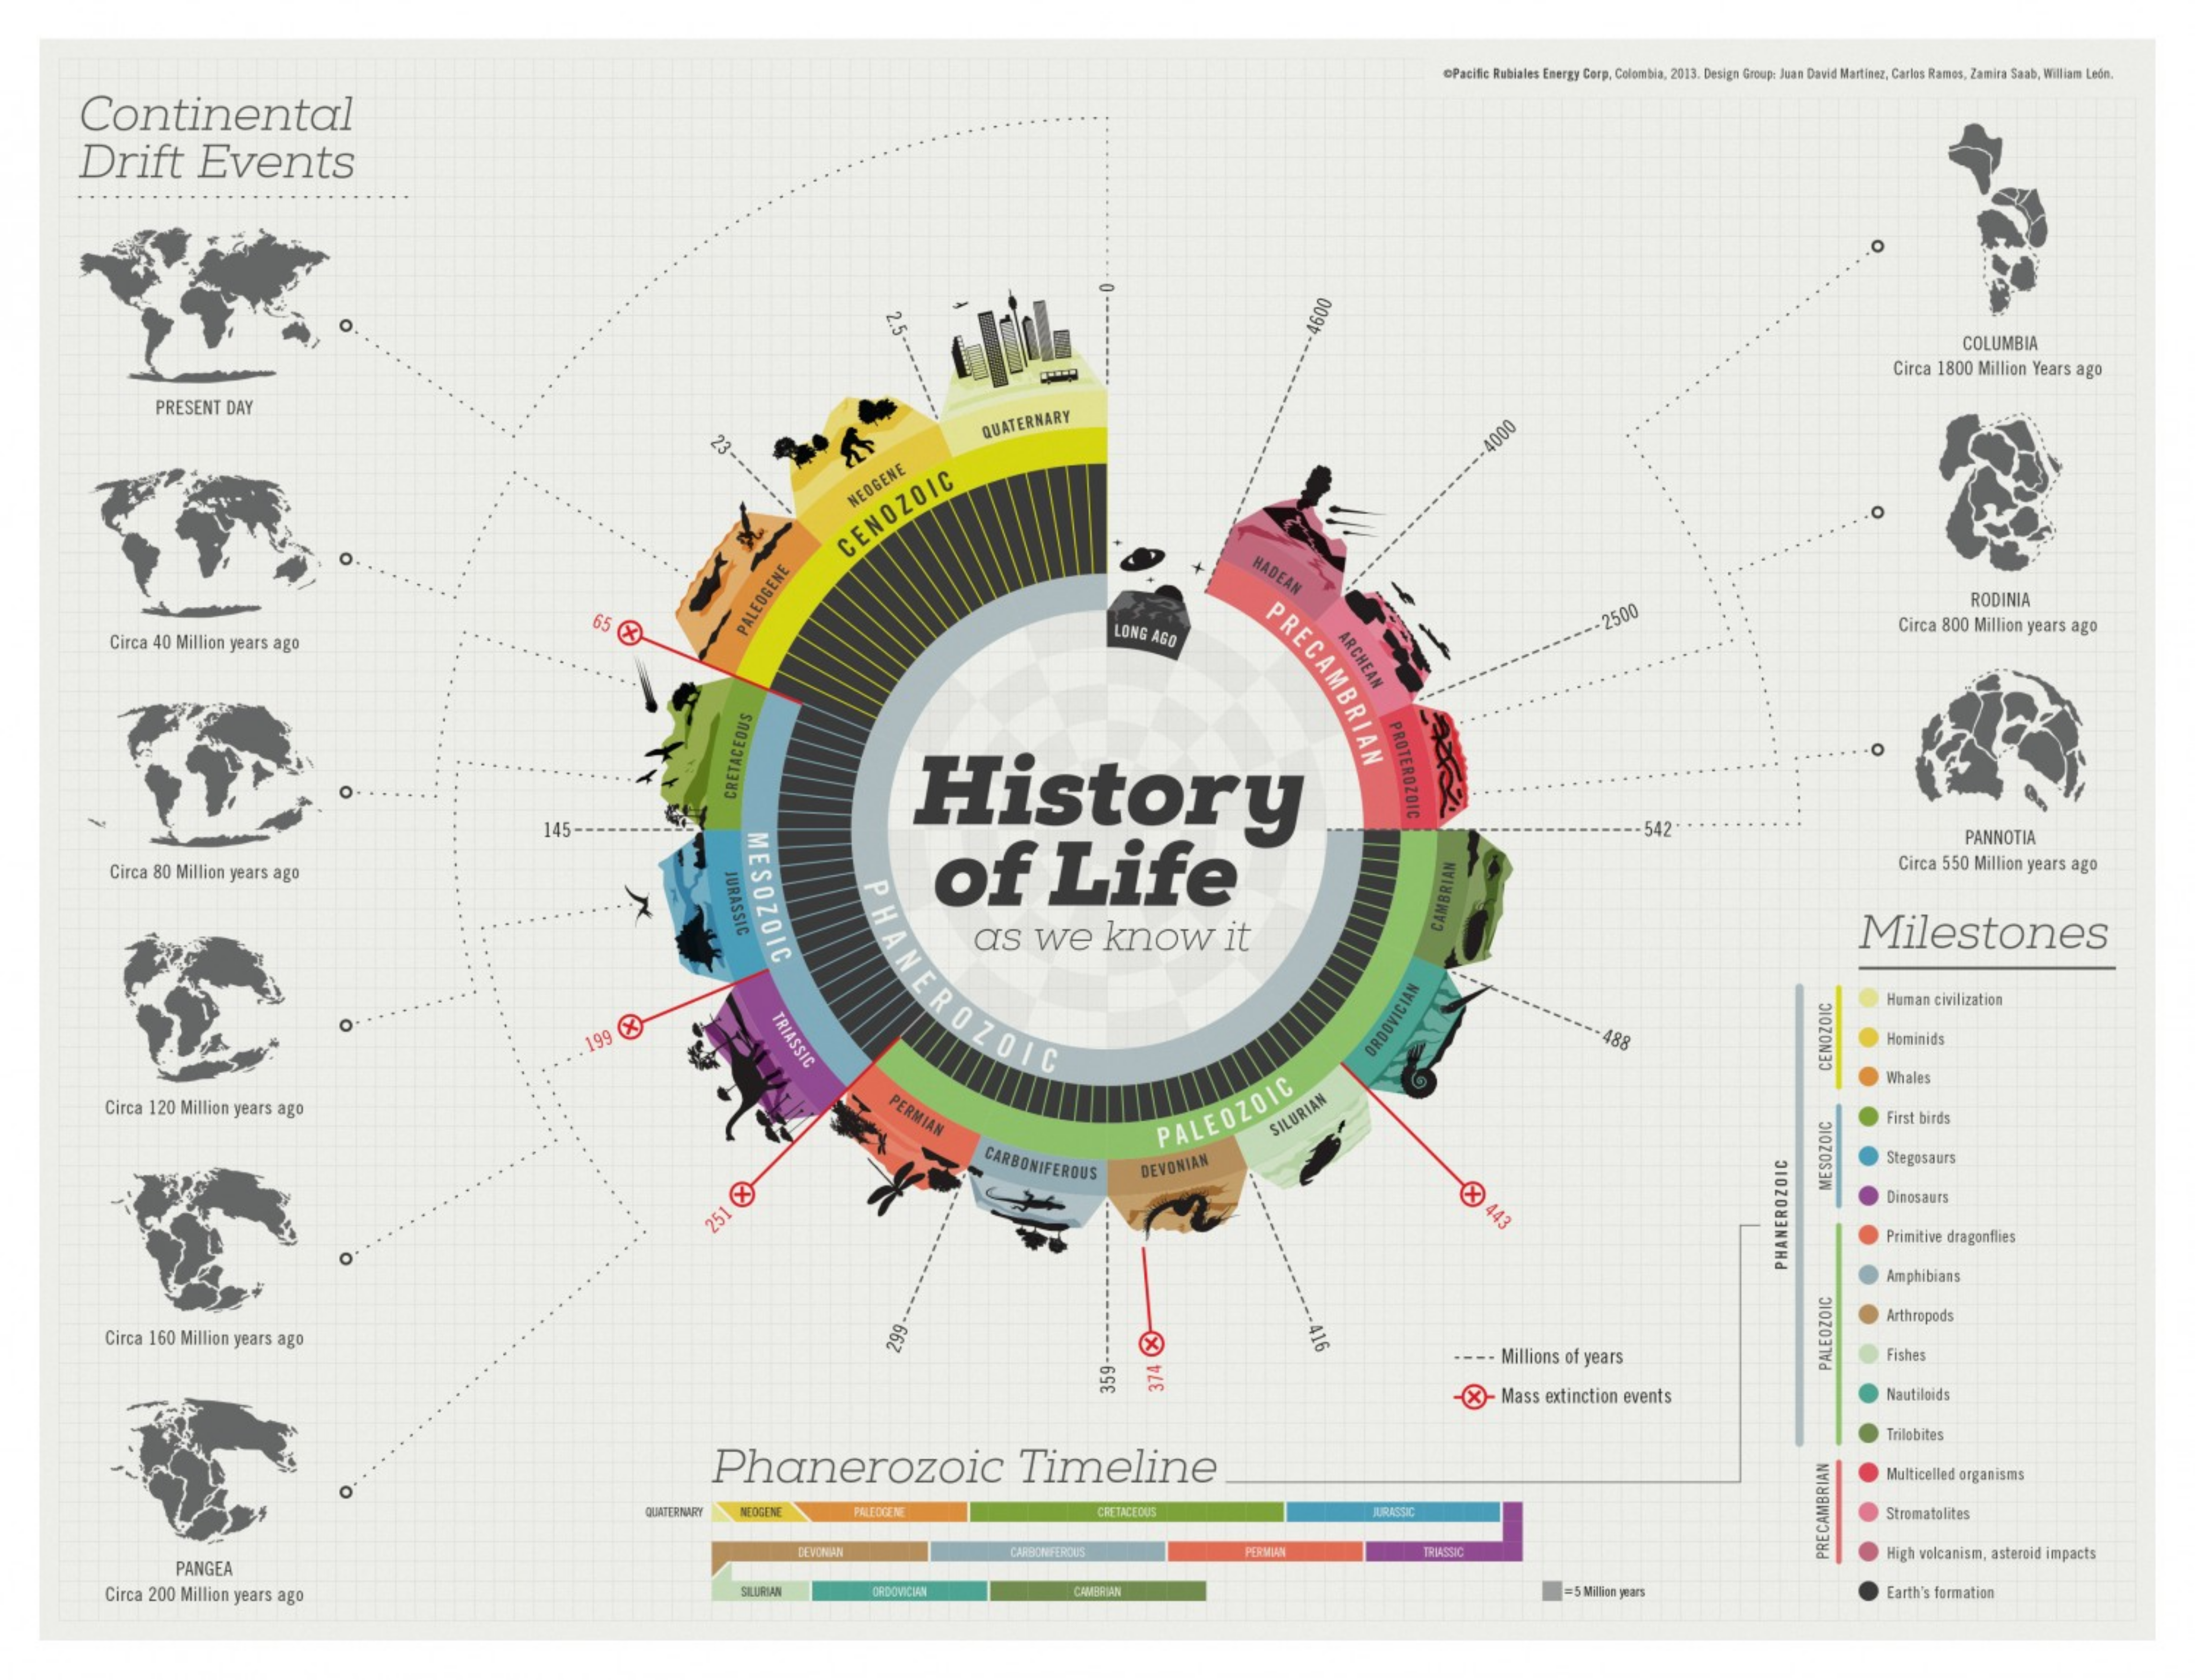
\includegraphics[width=3.3in]{History1.png}};
    \pause
    \node (img2) at (img1) {\includegraphics[width=3.3in]{History2.png}};
    \pause
    \node (img3) at (img1) {\includegraphics[width=3.3in]{History3.png}};
    \pause
    \node (img4) at (img1) {\includegraphics[width=3.3in]{History4.png}};
    \pause
    \node (img5) at (img1) {\includegraphics[width=3.3in]{History5.png}};
  \end{tikzpicture}
  \end{center}
  \vspace{-10pt}
  
  \begin{itemize}
    \item Mutualistic networks are almost as old as life itself
    \begin{itemize}
      \item \it Multi-cellularity possibly arose from a mutualism 
    \end{itemize}
  \end{itemize}
  
  \end{frame}

%%%%%%%%%%%%%%%%%%%%%%%%%%%%%%%%%%%%%%%%%%%%%%%%%%%%%
\begin{frame}{Why study Mutualistic Networks?}

\begin{columns}[c]
  \column{0.6\linewidth}
    \begin{itemize}[<+->]\setlength{\itemindent}{0em}\itemsep10pt
      \item Pollination services
      \item Ecosystem functioning
      \item Biodiversity loss 
    \end{itemize}
  \column{0.4\linewidth}\centering
  \includegraphics[width=.8\textwidth]{Pollination.jpg}	\\
  {\tiny Source: \url{https://morningchores.com/pollination}\par}
\end{columns}
\pause
\begin{center}
  \includegraphics[width=\textwidth]{seasonalnetwork(BBG).png}
  \includegraphics[width=\textwidth]{seasonalnetwork(IBGE).png}\\\tiny Rabeling et al PLoS One 2019  
\end{center}

\end{frame}  

%%%%%%%%%%%%%%%%%%%%%%%%%%%%%%%%%%%%%%%%%%%%%%%%%%%%%%
\begin{frame}[plain]{}
  \begin{center}
    \includegraphics[width = .8\textwidth]{HumHawkMoth.jpg}\\
    {\tiny \url{https://commons.wikimedia.org/w/index.php?curid=763031}\par }
  \end{center}
\end{frame}

%%%%%%%%%%%%%%%%%%%%%%%%%%%%%%%%%%%%%%%%%%%%%%%%%%%%%%
\section{\scshape Structure and Stability}
%%%%%%%%%%%%%%%%%%%%%%%%%%%%%%%%%%%%%%%%%%%%%%%%%%%%%%

%%%%%%%%%%%%%%%%%%%%%%%%%%%%%%%%%%%%%%%%%%%%%%%%%%%%%%
\begin{frame}{Structure and Stability}

  \begin{columns}[c]
    \column{0.85\linewidth}
      \begin{itemize}[<+->]\setlength{\itemindent}{0em}\itemsep6pt
        \item Most work has been done on Plant-Pollinator networks
        \begin{itemize}
          \item These are called ``bipartite'' networks because the nodes are at only two levels: Plants and Pollinators
        \end{itemize}
        \item {\it Nestedness} is considered to be an important feature for the system's {\it stability} and {\it resilience} (coming up)
        \item Interaction {\it generalization} vs {\it specialization} is also considered important (coming up)
        \item Mutualistic networks have {\it Modules}\footnotemark
        \begin{itemize}
          \item But modules in these systems are less easy to identify and are poorly understood
        \end{itemize} 

      \end{itemize}
    \column{0.15\linewidth}\centering
    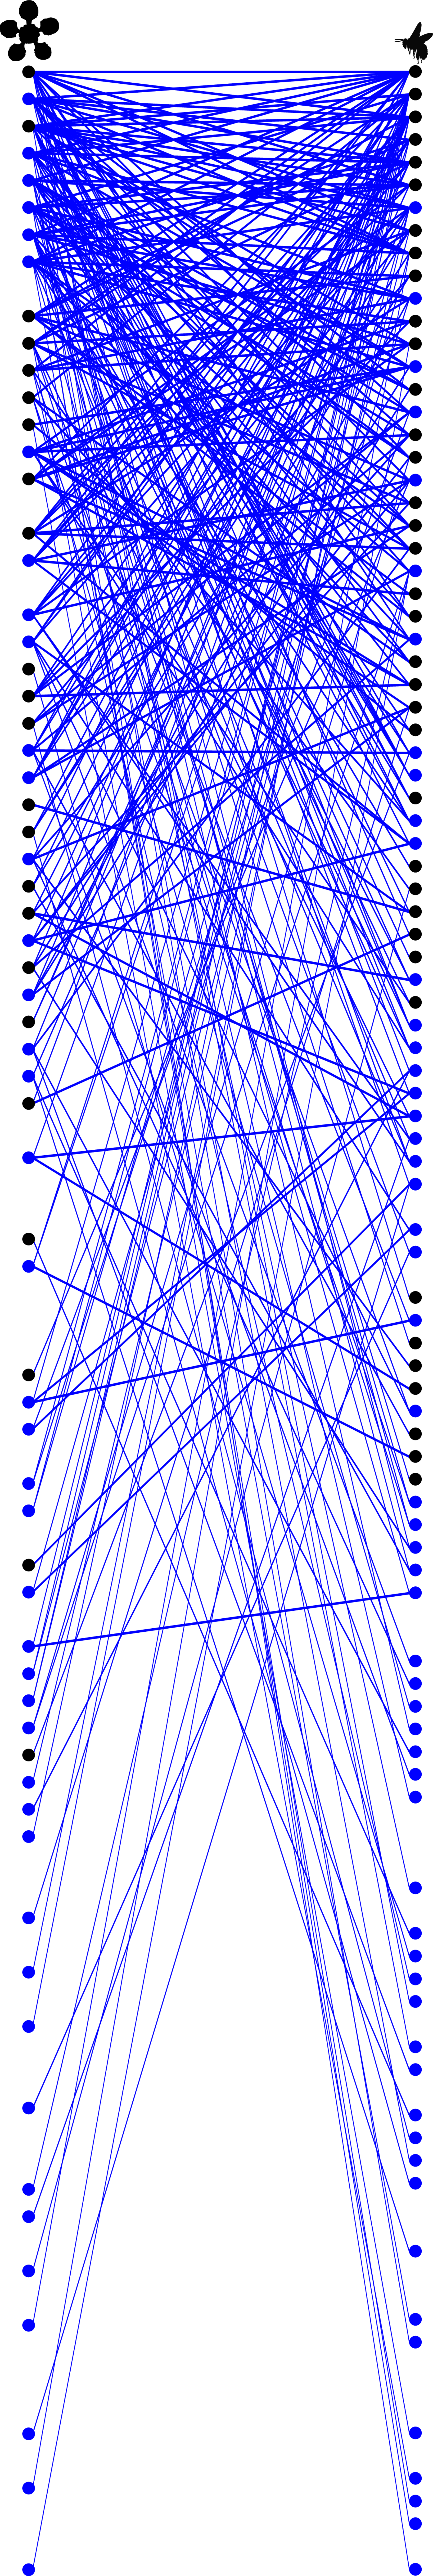
\includegraphics[width=.8\textwidth]{PolliNet.pdf}
  \end{columns}

\footnotetext{Like other ecological networks: Review lecture on Ecological Interaction Networks}

\end{frame}
    
%%%%%%%%%%%%%%%%%%%%%%%%%%%%%%%%%%%%%%%%%%%%%%%%%%%%%%
\begin{frame}{The role of nestedness}

  \begin{columns}[c]
    \column{0.6\linewidth}
      \begin{itemize}[<+->]\setlength{\itemindent}{0em}\itemsep10pt
        \item {\bf Nestedness of a network}: a network structural pattern where specialist pollinators species visit plant species that are subsets of those visited by more generalist pollinators 
        \item Means that the network has a ``strong'' core of highly connected generalists
        \begin{itemize} 
          \item A generalist pollinator visits and pollinates many different plant species (same criteria can be applied to plants)
        \end{itemize}  
      \end{itemize}

    \column{0.4\linewidth}\centering
    \includegraphics[width=\textwidth]{Nestedness.pdf}	\\
    {\tiny Pawar, Science 2015}
    \begin{itemize}
      \item Nestedness Illustrated: The network on the left is perfectly nested, while the one on the right is not
    \end{itemize}
  \end{columns}
\end{frame}

%%%%%%%%%%%%%%%%%%%%%%%%%%%%%%%%%%%%%%%%%%%%%%%%%%%%%%
\begin{frame}{The role of nestedness}

  \begin{columns}[c]
    \column{0.65\linewidth}
      \begin{itemize}[<+->]\setlength{\itemindent}{0em}\itemsep10pt
        \item Nestedness also means asymmetry in specialization: Specialist
        plants are pollinated by generalist animals, but generalist plants are
        pollinated by both specialist and generalist pollinators\footnotemark
        \item All these properties have been linked to {\it robustness} of pollination networks to species loss:
        \begin{itemize}
          \item If you remove a random  species in a more nested network, it is less likely to collapse
        \end{itemize}
      \end{itemize}
    \column{0.35\linewidth}\centering
    \includegraphics[width=\textwidth]{Robustness.pdf}	\\
    {\tiny Rabeling et al, PlOS One 2019}
  \end{columns}
  \begin{itemize} 
    \item \it But role of nestedness remains debated...
  \end{itemize}  
\footnotetext{In contrast to {\it reciprocal specialization} where specialist pollinators interact with specialist plants} 
\end{frame}

%%%%%%%%%%%%%%%%%%%%%%%%%%%%%%%%%%%%%%%%%%%%%%%%%%%%%%
\begin{frame}{Temporal variation in mutualistic networks}
  
  \begin{columns}[c]
    \column{0.72\linewidth}
      \begin{itemize}[<+->]\setlength{\itemindent}{0em}\itemsep6pt
        \item The structure of Mutualistic networks can change rapidly over time
        \item This issues is poorly understood, but very important
        \item These changes in network structure are linked to climate (and temperature)
        \item Climate change can disrupt such temporally changing networks (e.g., though {\it Phenological mismatches} between plants and pollinators)  
      \end{itemize}
      \pause
      \begin{center}
        \includegraphics[width=\textwidth]{seasonalnetwork(IBGE).png}\\\tiny Rabeling et al PLoS One 2019  
      \end{center}    
      \column{0.28\linewidth}\centering
    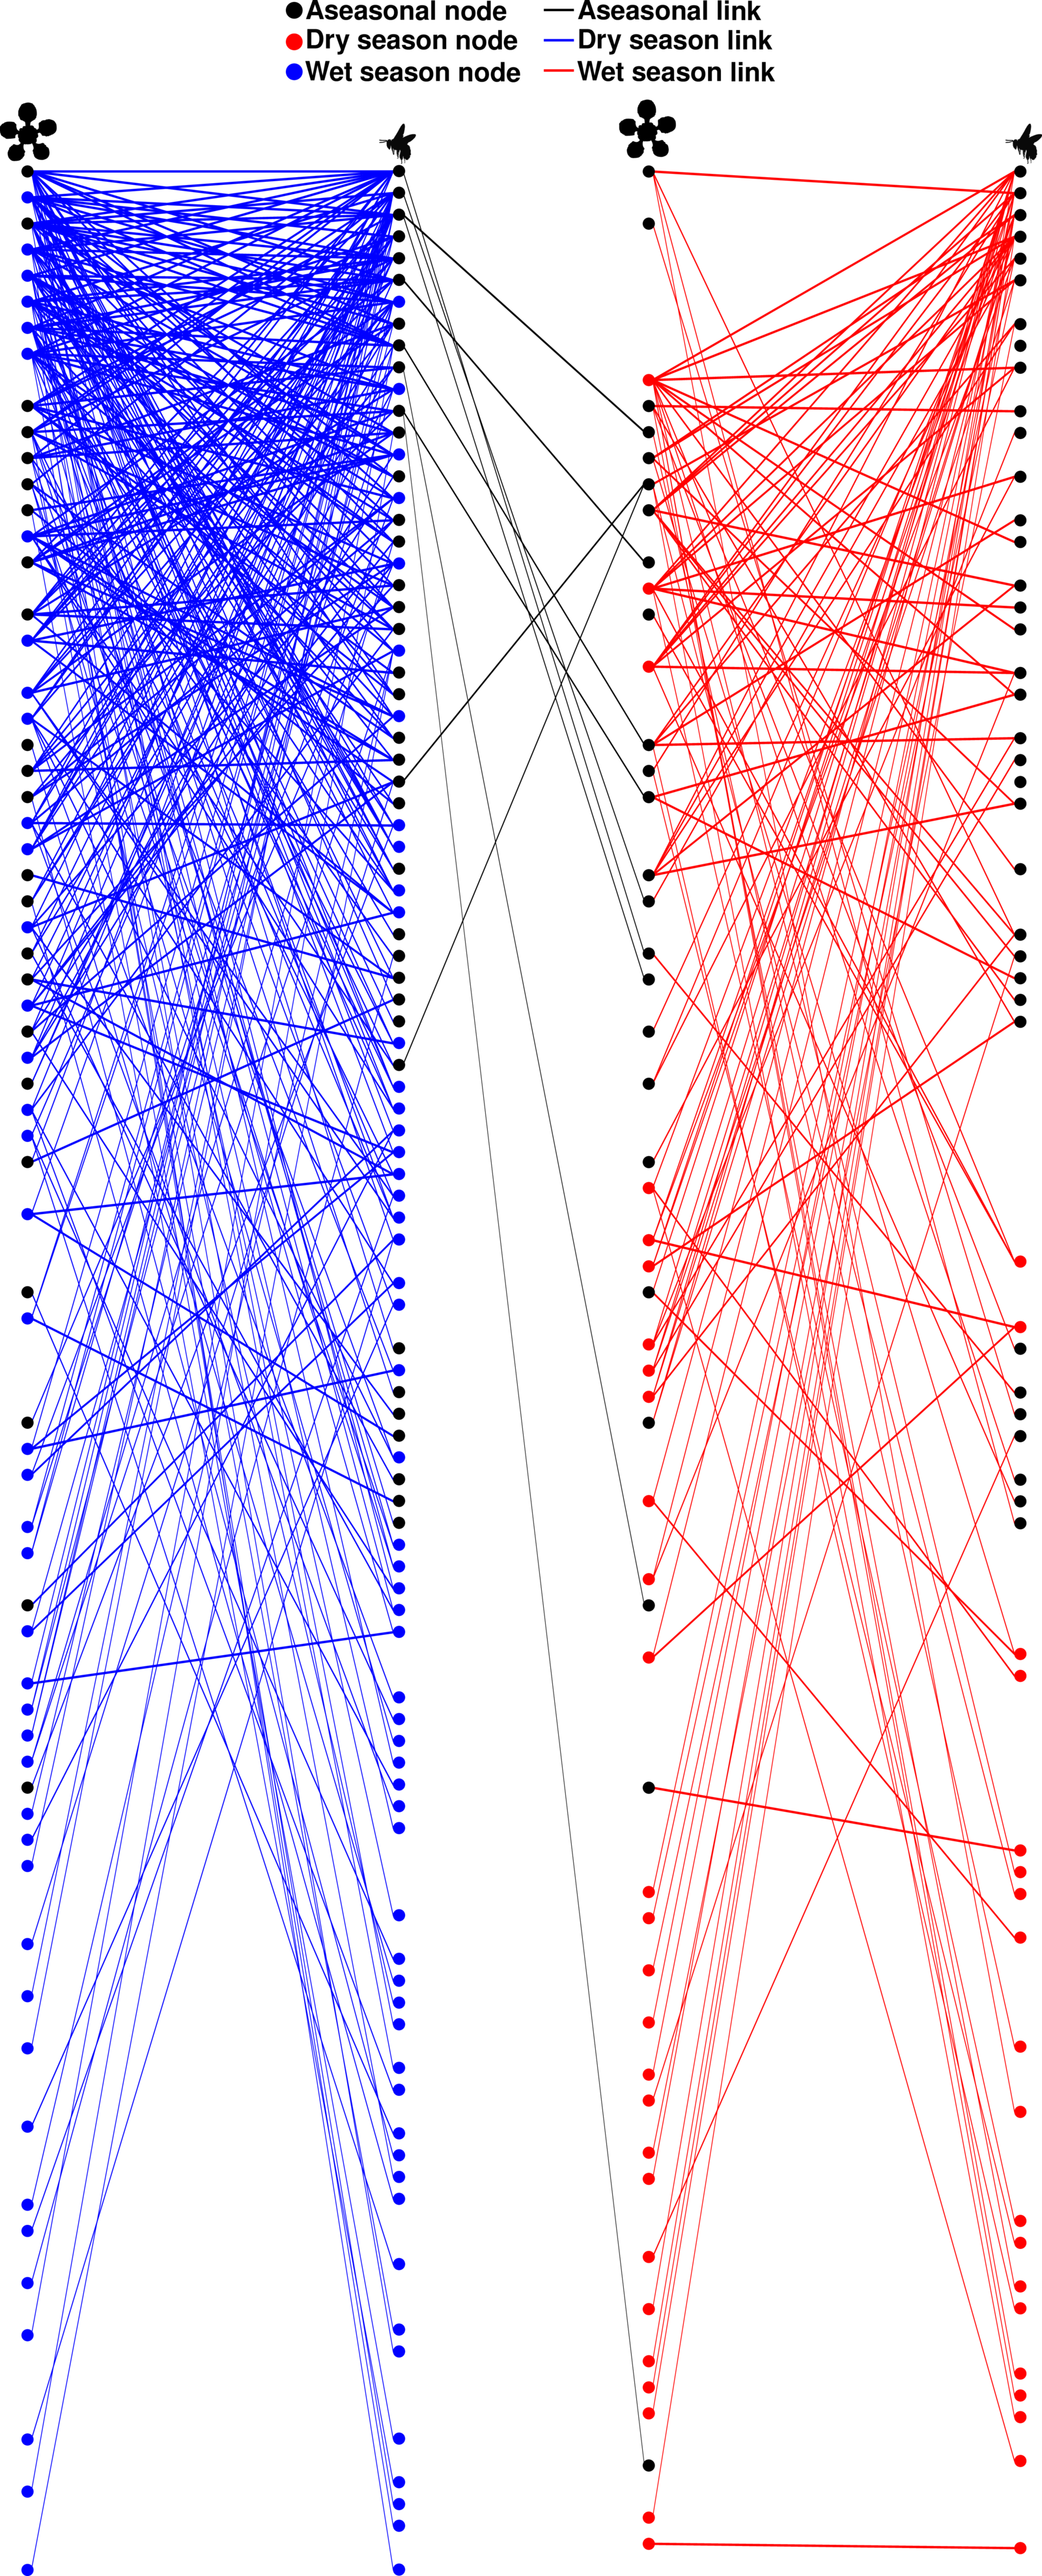
\includegraphics[width=\textwidth]{PolliNet_Seasonal.pdf}
  \end{columns}
\pause
\begin{center}
  \includegraphics[width=\textwidth]{seasonalnetwork(BBG).png}\\ 
  \tiny Rabeling et al PLoS One 2019  
\end{center}
\end{frame}

%%%%%%%%%%%%%%%%%%%%%%%%%%%%%%%%%%%%%%%%%%%%%%%%%%%%%%
\begin{frame}{Temporal variation in mutualistic networks}
  
\begin{center}
  \includegraphics[width=\textwidth]{Cerrado.jpg}\\ \tiny Gottsberger \& Silberbauer-Gottsberger, Acta Bot. Brasilica 2018  
\end{center}
\begin{center}
  \includegraphics[width=\textwidth]{seasonalnetwork(BBG).png}
  \includegraphics[width=\textwidth]{seasonalnetwork(IBGE).png}\\\tiny Rabeling et al PLoS One 2019  
\end{center}

\end{frame}

%%%%%%%%%%%%%%%%%%%%%%%%%%%%%%%%%%%%%%%%%%%%%%%%%%%%%%
\begin{frame}{Temporal variation in mutualistic networks}
  
  \begin{center}
    \includegraphics[width=\textwidth]{Cerrado_polli.jpg}\\ \tiny Souza et al. J. Ecol. 2018  
  \end{center}
  \end{frame}

%%%%%%%%%%%%%%%%%%%%%%%%%%%%%%%%%%%%%%%%%%%%%%%%%%%%%%
\begin{frame}{Microbial mutualistic networks}
  
  \begin{columns}[c]
    \column{0.65\linewidth}
      \begin{itemize}[<+->]\setlength{\itemindent}{0em}\itemsep3pt
        \item Microbial networks are important model systems for understanding mutualism vs competition   
        \item In fact, the interaction network in microbial communities can go from being competitive to mutualistic in a matter of days to months! 
        \item Increasing mutualism increases the rate of microbial community functioning (e.g., decomposition of leaf litter)
        \item Temperature can accelerate this effect\footnotemark
      \end{itemize}
    \column{0.35\linewidth}\centering
    \includegraphics[width=\textwidth]{Microbial_Mutualism.pdf}\\
    \vspace{-6pt}
    {\tiny Lawrence et al PLoS Biology 2012}\\
    \includegraphics[width=\linewidth]{Bacteria_Net.png}\\
    \vspace{-6pt}
    {\tiny Goldford et al Science 2018}
 
  \end{columns}

  \footnotetext{Review lectures on Energy and Metabolism as well as Consumer-Resource Interactions  }

\end{frame}
%%%%%%%%%%%%%%%%%%%%%%%%%%%%%%%%%%%%%%%%%%%%%%%%%%%%%%
\section{\scshape Summary}
%%%%%%%%%%%%%%%%%%%%%%%%%%%%%%%%%%%%%%%%%%%%%%%%%%%%%%
  \begin{frame}{Summary}
  
    \begin{itemize}[<+->] \setlength{\itemindent}{0em} \itemsep10pt
      \item Mutualistic networks are important for many ecosystem ``services'' (e.g., pollination)
      
      \item The structure of mutualistic networks affects their stability, resilience, and robustness  
        
      \item Nestedness is believed to enhance the robustness (and stability) of mutualistic networks  (but this is still debated)

      \item Plant-Pollinator networks can change over time (but this is poorly understood)
      
      \item Microbial networks can rapidly switch from being competitive to cooperative (mutualistic) over time
    \end{itemize}
  
  \end{frame}  

%%%%%%%%%%%%%%%%%%%%%%%%%%%%%%%%%%%%%%%%%%%%%%%%%%%%%%
\begin{frame}{Discussion Questions}

  \begin{enumerate}\setlength{\itemindent}{-1em}\itemsep4pt
    
    \item What are the differences between trophic (e.g., food web) and mutualistic networks?
    
    \item Can we truly study Mutualistic and Trophic networks separately?
    
    \item What role might body size play in Mutualistic (e.g., plant-pollinator) networks? 
    
    \item How do you thing global climate change might affect plant-pollinator networks and pollination services? 
      
    \item How do you think increasing mutualism increases the rate of microbial
    community functioning (e.g., decomposition of leaf litter)? What role can
    temperature play in this? How does this relate to the global carbon cycle?
    (Hint: Leaf litter decomposition releases CO$_2$ )
  \end{enumerate}

\end{frame}

  
%%%%%%%%%%%%%%%%%%%%%%%%%%%%%%%%%%%%%%%%%%%%%%%%%%%%%%
\begin{frame}{Readings}

\begin{enumerate}\setlength{\itemindent}{-2em}\itemsep4pt

  \item Bascompte, J. \& Jordano, P. Plant-animal mutualistic networks: The architecture of biodiversity. Annual Review of Ecology Evolution and Systematics 38, 567--593 (2007).
  
  % \item Bastolla, U. et al. The architecture of mutualistic networks minimizes competition and increases biodiversity. Nature 458, 101--1020 (2009)
 
  \item Th\'{e}bault, E. \& Fontaine, C. Stability of ecological communities and the architecture of mutualistic and trophic networks. Science. 329, 853--856 (2010).
 
  \item Rabeling, S. C. et al. Seasonal variation of a plant-pollinator network in the Brazilian Cerrado: Implications for community structure and robustness. PLoS One 14, (2019).
  
  \item  Tylianakis, J. M.,  et al. Conservation of species interaction networks. Biological Conservation 143, 2270--2279 (2010).
  % \item Pawar, S. Why are plant-pollinator networks nested? Science. 345, 383 (2014).
  
  \item Lawrence, D. et al. Species interactions alter evolutionary responses to a novel environment. PLoS Biol. 10, e1001330 (2012).

\end{enumerate}
  
\end{frame}

\end{document}